
%(BEGIN_QUESTION)
% Copyright 2010, Tony R. Kuphaldt, released under the Creative Commons Attribution License (v 1.0)
% This means you may do almost anything with this work of mine, so long as you give me proper credit

This single-loop control system has a problem: the pressure indicated on the controller's faceplate only shows 45 inches W.C. despite the setpoint's value of 95 inches W.C. (measurement range = 0 to 120 inches W.C.).  The operator has already attempted to correct the problem by placing the controller in manual and setting the output at 100\%, to no avail:

$$\includegraphics[width=15.5cm]{i01590x01.eps}$$

Determine the diagnostic value of each of the following tests.  Assume only one fault in the system, including any single component or any single wire/cable/tube connecting components together.  If a proposed test could provide new information to help you identify the location and/or nature of the one fault, mark ``yes.''  Otherwise, if a proposed test would not reveal anything relevant to identifying the fault (already discernible from the measurements and symptoms given so far), mark ``no.''

% No blank lines allowed between lines of an \halign structure!
% I use comments (%) instead, so that TeX doesn't choke.

$$\vbox{\offinterlineskip
\halign{\strut
\vrule \quad\hfil # \ \hfil & 
\vrule \quad\hfil # \ \hfil & 
\vrule \quad\hfil # \ \hfil \vrule \cr
\noalign{\hrule}
%
% First row
{\bf Diagnostic test} & {\bf Yes} & {\bf No} \cr
%
\noalign{\hrule}
%
% Another row
Measure AC line voltage &  &  \cr
%
\noalign{\hrule}
%
% Another row
Measure DC power supply output voltage &  &  \cr
%
\noalign{\hrule}
%
% Another row
Inspect PID tuning parameters in controller &  &  \cr
%
\noalign{\hrule}
%
% Another row
Inspect PV range values (LRV, URV) in controller &  &  \cr
%
\noalign{\hrule}
%
% Another row
Push flapper toward nozzle in I/P &  &  \cr
%
\noalign{\hrule}
%
% Another row
Pull flapper away from nozzle in I/P &  &  \cr
%
\noalign{\hrule}
%
% Another row
Measure DC voltage between TB1-3 and TB1-4 &  &  \cr
%
\noalign{\hrule}
%
% Another row
Measure DC voltage between TB1-6 and TB1-7 &  &  \cr
%
\noalign{\hrule}
} % End of \halign 
}$$ % End of \vbox


\underbar{file i01590}
%(END_QUESTION)





%(BEGIN_ANSWER)

\noindent
{\bf Partial answer:}

% No blank lines allowed between lines of an \halign structure!
% I use comments (%) instead, so that TeX doesn't choke.

$$\vbox{\offinterlineskip
\halign{\strut
\vrule \quad\hfil # \ \hfil & 
\vrule \quad\hfil # \ \hfil & 
\vrule \quad\hfil # \ \hfil \vrule \cr
\noalign{\hrule}
%
% First row
{\bf Diagnostic test} & {\bf Yes} & {\bf No} \cr
%
\noalign{\hrule}
%
% Another row
Measure AC line voltage &  &  \cr
%
\noalign{\hrule}
%
% Another row
Measure DC power supply output voltage &  & $\surd$ \cr
%
\noalign{\hrule}
%
% Another row
Inspect PID tuning parameters in controller &  &  \cr
%
\noalign{\hrule}
%
% Another row
Inspect PV range values (LRV, URV) in controller &  &  \cr
%
\noalign{\hrule}
%
% Another row
Push flapper toward nozzle in I/P &  &  \cr
%
\noalign{\hrule}
%
% Another row
Pull flapper away from nozzle in I/P &  & \cr
%
\noalign{\hrule}
%
% Another row
Measure DC voltage between TB1-3 and TB1-4 &  & $\surd$ \cr
%
\noalign{\hrule}
%
% Another row
Measure DC voltage between TB1-6 and TB1-7 &  &  \cr
%
\noalign{\hrule}
} % End of \halign 
}$$ % End of \vbox

%(END_ANSWER)





%(BEGIN_NOTES)

% No blank lines allowed between lines of an \halign structure!
% I use comments (%) instead, so that TeX doesn't choke.

$$\vbox{\offinterlineskip
\halign{\strut
\vrule \quad\hfil # \ \hfil & 
\vrule \quad\hfil # \ \hfil & 
\vrule \quad\hfil # \ \hfil \vrule \cr
\noalign{\hrule}
%
% First row
{\bf Diagnostic test} & {\bf Yes} & {\bf No} \cr
%
\noalign{\hrule}
%
% Another row
Measure AC line voltage &  & $\surd$ \cr
%
\noalign{\hrule}
%
% Another row
Measure DC power supply output voltage &  & $\surd$ \cr
%
\noalign{\hrule}
%
% Another row
Inspect PID tuning parameters in controller &  & $\surd$ \cr
%
\noalign{\hrule}
%
% Another row
Inspect PV range values (LRV, URV) in controller &  & $\surd$ \cr
%
\noalign{\hrule}
%
% Another row
Push flapper toward nozzle in I/P & $\surd$ &  \cr
%
\noalign{\hrule}
%
% Another row
Pull flapper away from nozzle in I/P &  & $\surd$ \cr
%
\noalign{\hrule}
%
% Another row
Measure DC voltage between TB1-3 and TB1-4 &  & $\surd$ \cr
%
\noalign{\hrule}
%
% Another row
Measure DC voltage between TB1-6 and TB1-7 & $\surd$ &  \cr
%
\noalign{\hrule}
} % End of \halign 
}$$ % End of \vbox


\vfil \eject


$$\includegraphics[width=15.5cm]{i01590x02.eps}$$


\filbreak \vskip 20pt \vbox{\hrule \hbox{\strut \vrule{} {\bf Virtual Troubleshooting} \vrule} \hrule}

\noindent
{\bf Predicting the effect of a given fault:} present each of the following faults to the students, one at a time, having them comment on all the effects each fault would produce.

\begin{itemize}
\item{} 
\item{} 
\item{} 
\end{itemize}


\vskip 10pt


\noindent
{\bf Identifying possible/impossible faults:} present symptoms to the students and then have them determine whether or not a series of suggested faults could account for all the symptoms, explaining {\it why} or {\it why not} for each proposed fault:

\begin{itemize}
\item{} Symptom: {\it Gauge reads 110 inches WC even with SP set to 80 inches WC}
\item{} Controller left in manual mode? {\it possible}
\item{} Transmitter calibration error (reads too high)? {\it impossible}
\item{} Transmitter calibration error (reads too low)? {\it possible}
\item{} Valve V1 shut? {\it possible}
\item{} Air supply to control valve failed? {\it impossible}
\item{} I/P coil failed open? {\it impossible}
\item{} I/P coil failed shorted? {\it impossible}
\item{} 250 ohm resistor failed open? {\it impossible}
\end{itemize}


\vskip 10pt


\noindent
{\bf Determining the utility of given diagnostic tests:} present symptoms to the students and then propose the following diagnostic tests one by one.  Students rate the value of each test, determining whether or not it would give useful information (i.e. tell us something we don't already know).  Students determine what different results for each test would indicate about the fault, if anything:

\begin{itemize}
\item{} Symptom: {\it }
\item{}  -- {\bf Yes/No}
\item{}  -- {\bf Yes/No}
\end{itemize}


\vskip 10pt


\noindent
{\bf Diagnosing a fault based on given symptoms:} imagine the ??? fails ??? in this system (don't reveal the fault to students!).  Present the operator's observation(s) to the students, have them consider possible faults and diagnostic strategies, and then tell them the results of tests they propose based on the following symptoms, until they have properly identified the nature and location of the fault:

\begin{itemize}
\item{} {\it }
\item{} 
\item{} 
\end{itemize}

%INDEX% Troubleshooting review: electric circuit diagnostic test usefulness

%(END_NOTES)


